
\chapter{Minimality -- some observations and some challenges}
\label{sec:minim-some-observ}

The previous chapter provided a constructive answer to the question of how to build a Deterministic Suffix-reading Automaton from a DFA. The derivation procedure, based on suffix-tracking sets, can generate a language-equivalent DSA. However, the choice of a suffix-tracking set is not unique, meaning our procedure can produce many different DSAs for the same language, each with a different total size. This naturally gives rise to the fundamental optimization problem: how do we find a DSA that is minimal, that is, one with the smallest possible total size?

In classical automata theory, the path to a minimal DFA is well-trodden, anchored by the Myhill-Nerode theorem and the existence of a unique canonical DFA for every regular language. One might reasonably expect a similar principle to apply here: that a minimal DSA could be found by applying our derivation procedure to this canonical DFA. This chapter will demonstrate that DSA minimization is far more complex and challenges these classical intuitions.

We begin by establishing that unlike DFAs, minimal DSAs are not necessarily unique. We then present the central, surprising observation of this chapter: we will show via a concrete counterexample that the smallest DSA derivable from the canonical DFA of a language is not always a minimal DSA for that language. In some cases, a smaller DSA can only be derived from a larger, non-minimal DFA. This finding has profound implications, suggesting that the standard Nerode equivalence does not capture the right notion of state equivalence for DSA minimization.

This investigation will proceed in three parts. First, we will explore these counter-intuitive properties. Second, we will formalize the inherent difficulty of this problem by proving that DSA minimization is NP-complete. Finally, in response to this complexity, we will introduce and analyze a well-behaved and practical subclass, `Strongly Deterministic Suffix-reading Automata (sDSAs)', for which the desirable link to the canonical DFA is restored.

%marker
\vspace{.25cm}

Theorem~\ref{thm:comparing-dsa-with-dfa-dga} shows that we cannot
expect DSAs to be smaller than (trim) DFAs or DGAs in
general. However, Lemma~\ref{lem:dsa-small} and
Figure~\ref{fig:if-else} show that there are cases where DSAs are
smaller and more readable. This motivates us to ask the question of
how we can find a minimal DSA, that is, a DSA of the smallest (total)
size. The first observation is that minimal DSAs need not be unique
--- see Figure~\ref{fig:no-canonical}.

\begin{lemma}
   \label{lem:no-canonical}
   The minimal DSA need not be unique.
 \end{lemma}
\begin{proof}
  Figure~\ref{fig:no-canonical} illustrates two DSAs, both of size $7$ ($2$ states,
  $2$ edges, total label length $3$), accepting
  the same language. From DSA $\Aa_1$, we can see that the
  language accepted is $b^*a^*abb^*a$. From DSA $\Aa_2$, we can derive
  the expression $b^*aa^*b^*ba$. It is easy to see that both the
  expressions are equivalent.

  It remains to show that there is no DSA of smaller
  size for this language. Let $L = b^*a^*abb^*a = b^*aa^*b^*ba$. Let
  $\Aa$ be a minimal automaton for $L$. Any
  DSA for $L$ has an initial state $q_0$ which is non-accepting (since
  $\e \notin L$, and an accepting state $q_1$ $\neq q_0$). So, in
  particular $\Aa$ has at least two states $q_0, q_1$. The
  smallest word in $L$ is $aba$. Suppose the accepting run of $\Aa$ on
  $aba$ is due to a transition $t:= q_0 \xra{aba} q_1$. Consider the word
  $abba \in L$. Transition $t$ does not match $abba$. Therefore, the
  first transition in the accepting run of $\Aa$ on $abba$ is some
  transition $t' \neq t$. This transition $t'$ will have a label of
  size at least $1$. Hence, $\Aa$ has at least two states, and at
  least two transitions: $t$ which contributes to size $4$ (includes
  $1$ edge and label of length $3$) and a transition $t'$ of size at
  least $2$. Therefore $|\Aa| \ge 2 + 4 + 2 = 8$, which is strictly
  greater than $|\Aa_1|$ and $|\Aa_2|$. This is a
  contradiction. Therefore the accepting run of $\Aa$ on $aba$ has a
  first transition on a prefix of $aba$, either $a$ or $ab$,
  corresponding to an intermediate transition $q_0 \xra{a} q'$ or $q_0
  \xra{ab} q'$. In the former case, there can be a transition $q'
  \xra{ba} q_1$ to accept $aba$ (if the transition is on just $b$, it only makes the automaton larger since $a$ remains to be read), and in the latter case, a transition
  $q' \xra{a} q_1$. This gives the two automata $\Aa_2$ and $\Aa_1$,
  which are therefore indeed minimal.
\end{proof}

The next  observation
is that a minimal DSAs will be well-formed: if there are two transitions
$q \xra{\a} q_1$ and $q \xra{\beta_1 \a \beta_2} q_2$, then we can remove
the second transition since it will never get fired.

\begin{figure}[t]
  \centering
  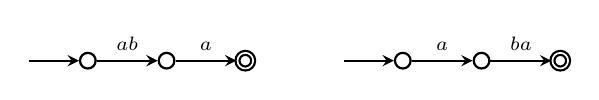
\begin{tikzpicture}[state/.style={circle, draw, thick, inner sep =
      2pt}]
    \begin{scope}[every node/.style={state}]
      \node (0) at (0,0) {}; \node (1) at (1, 0) {}; \node [double]
      (2) at (2, 0) {};
    \end{scope}
    \begin{scope}[->,>=stealth, thick, auto]
      \draw (-0.75, 0) to (0); \draw (0) to node {\scriptsize $ab$}
      (1); \draw (1) to node {\scriptsize $a$} (2);
    \end{scope}
    \begin{scope}[xshift=4cm]
      \begin{scope}[every node/.style={state}]
        \node (0) at (0,0) {}; \node (1) at (1, 0) {}; \node [double]
        (2) at (2, 0) {};
      \end{scope}
      \begin{scope}[->,>=stealth, thick, auto]
        \draw (-0.75, 0) to (0); \draw (0) to node {\scriptsize $a$}
        (1); \draw (1) to node {\scriptsize $ba$} (2);
      \end{scope}
    \end{scope}
  \end{tikzpicture}
  \caption{Minimal DSA is not unique}
  \label{fig:no-canonical}
\end{figure}



Due to the ``well-formedness'' property in
suffix-tracking sets, the DSAs induced by suffix-tracking sets are
naturally well-formed. Furthermore, since removing redundant transitions preserves
this property, the DSAs that are derived using our DFA-to-DSA
procedure (Definition~\ref{def:derived-dsa}) are well-formed. The next
proposition shows that every DSA that is well-formed and has no
redundant transitions (and in particular, the minimal
DSAs) can be derived from the corresponding tracking DFAs.


\begin{restatable}{proposition}{dsaDerivableFromTracking}
  \label{prop:dsa-derivable-from-tracking-dfa}
  Every well-formed DSA with no redundant transitions can
  be derived from its tracking DFA.
\end{restatable}

\begin{proof}
  We use notation as in Definition~\ref{def:notation}.
  Consider a DSA $\Aa$ that is well-formed and has no redundant
  bigger-suffix-transitions. Let $M_\Aa$ be its tracking DFA as in
  Definition~\ref{def:tracking-dfa}. Let $S = \bigcup_{q\in\Aa}
  {(q,\e)}$. Here is the schema of the proof:
  \begin{align*}
  M_\Aa \xra{~~S~~} \text{ induced DSA } \Aa' \xra{~~\text{remove redundant transitions~~}} \Aa
  \end{align*}
  \begin{enumerate}
  \item We first show that $S$ is suffix-tracking and well-formed.
  \item For each state $q$ of $\Aa$, and for each $\alpha \in \spaths{(q,\epsilon)}{S}$, either $\alpha \in \out(q)$ (a transition out of $q$ in $\Aa$) or $\alpha$ is a redundant bigger-suffix-transition that will be removed in the second step. 
  \end{enumerate}
  All together, this shows that $\Aa$ is derived from $M_\Aa$ using our procedure.

  
  \paragraph*{$S$ is suffix-tracking.} 
  Pick a state $(q, \beta)$ with $\beta \neq \e$. What is the set
  $\spath{(q, \e)}{(q, \beta)}{S}$? Clearly, $\beta \in \spath{(q,
    \e)}{(q, \beta)}{S}$. Let $\a \in \spath{(q,
    \e)}{(q, \beta)}{S}$, with $\a \neq \beta$. Then there is a path
  $(q, \e) \xra{\a_1} (q, \beta_1) \xra{\a_2} (q, \beta_2) \cdots (q, \beta_{k-1})
  \xra{\a_k} (q, \beta_k) = (q, \beta)$. Let $j \in \{1, \dots, k\}$
  be the largest index such that $\beta_j, \beta_{j+1}, \dots,
  \beta_k$ are all prefixes of $\beta$. Therefore, $\a$ starts by visiting a
  branch different from the prefixes of $\beta$, moves to potentially
  different ``branches'' (prefixes of other words in $\out(q)$, and on
  $\a_1 \dots 
  \a_j$ hits the $\beta$ branch, after which it stays in the same
  branch. By definition, $\beta_j$ is the longest prefix among
  $\outp(q)$ such that $\beta_j \sfx \a_1 \dots \a_j$. We can infer
  the following: (1) $\beta \sfx \a$, and (2) among $\outp(q)$,
  $\beta$ is the longest suffix of $\a$: otherwise, for $\a_1 \dots
  \a_j$, there would be a $\beta' \neq \beta_j$ which is a longer
  suffix, contradicting the definition of the transition $(q,
  \beta_{j-1}) \xra{\a_j} (q, \beta_j)$. 

  These observations are helpful to show that $S$ is
  suffix-tracking. Consider a transition $(q, \beta) \xra{a} (q,
  \beta')$ with $\beta' \neq \e$. We require to show that for every
  $\a \in \spath{(q, \e)}{(q, \beta)}{S}$, the longest suffix of $\a
  a$ among $\spaths{(q, \e)}{S}$ lies in $\spath{(q, \e)}{(q,
    \beta')}{S}$. Pick $\a \in \spath{(q, \e)}{(q, \beta)}{S}$, and
  consider the extension $\a a$. By (1) above, we have $\beta \sfx
  \a$. Since $\beta' \sfx \beta a$, we have $\beta' \sfx \a
  a$. Suppose there is an $\a'' \in \spath{(q, \e)}{(q, \beta'')}{S}$
  such that $|\a''| > |\beta'|$ and $\a'' \sfx \a a$. By definition of
  the transition $(q, \beta) \xra{a} (q,
  \beta')$, $\beta'$ is the longest suffix of $\beta a$, and hence
  $|\beta'| > |\beta''|$. From $|\a''| > |\beta'|$, $\a'' \sfx \a a$
  and $\beta' \sfx \beta a$, we have $\beta' \sfx \a''$. By point (2)
  of the above paragraph,  we have $|\beta''| > |\beta'|$. A
  contradiction. Therefore, there is no such $\a''$. Hence $\beta'$ is
  indeed the longest suffix of $\a a$ for all $\a \in \spath{(q,
    \e)}{(q, \beta)}{S}$.

  Now, consider a transition $(q, \beta) \xra{a} (q,\overline{\epsilon})$. This
  happens when no non-empty word in $\outp(q)$ is a suffix of $\beta
  a$. In that case, there is a transition $(q, \e) \xra{a} (q,\overline{\epsilon})$,
  and $a$ is indeed the longest suffix of $\beta a$ among $\spaths{(q,
    \e)}{S}$. This shows that every transition is suffix-compatible. 
 
	
  \paragraph*{$S$ is well-formed.} $S$ is well-formed naturally since $\Aa$ is well-formed. Suppose it
  was not. That means there exist states
  $p \in S, q' \notin S, q$, and words $\alpha \in \spath{p}{q}{S}, \beta'
  \in \spath{p}{q'}{S}$, such that $\alpha \sfx \beta'$. Then there is a state $q'' \in S$, and a word $\beta \in \spath{p}{q''}{S}$ such that
  $\beta' \pprfx \beta$, and we have $\a \sfx \beta'$. Since
  $\a,\beta \in \out(p)$, this means $\Aa$ is not well-formed, which is a
  contradiction.

  \paragraph*{Extra strings in the induced DSA are redundant.} In the induced DSA, we will have $\spaths{(q, \e)}{S}$ to have more
  words than $\out(q)$. We need to show that all the other words are
  redundant bigger-suffix-transitions, and hence will be removed by the
  derivation procedure. Consider a transition of the form $(q, \beta)
  \xra{a} (q', \e)$. For every word $\a \in \spath{(q, \e)}{(q,
    \beta)}{S}$, with $|\a| > |\beta|$, we have $\beta$ as the longest
  suffix of $\a$, among $\outp(q)$. Therefore, there is no $\beta'$
  with $|\a| \ge |\beta'| > |\beta|$ with $\beta' \sfx \a$. This is
  sufficient to see that there is no $\beta' a \in \out(q)$ such that
  $\beta a \sfx \beta' a \sfx \a a$. Hence $\a a$ is a redundant
  bigger-suffix-transition in the induced DSA.

  By assumption, we have no redundant bigger-suffix-transitions in
  $\Aa$. Hence, in the derivation procedure, we do not remove any
  transition already present in $\Aa$. This shows that the finally derived DSA is exactly $\Aa$. 
\end{proof}
 

Proposition~\ref{prop:dsa-derivable-from-tracking-dfa} says that if we
somehow had access to the tracking DFA of a minimal DSA, we will be
able to derive it using our procedure. The challenge however is that
this tracking DFA may not necessarily be the canonical DFA for the
language. In fact, we now show that a smallest DSA that can be derived
from the canonical DFA need not be a minimal DSA.

\begin{figure}
  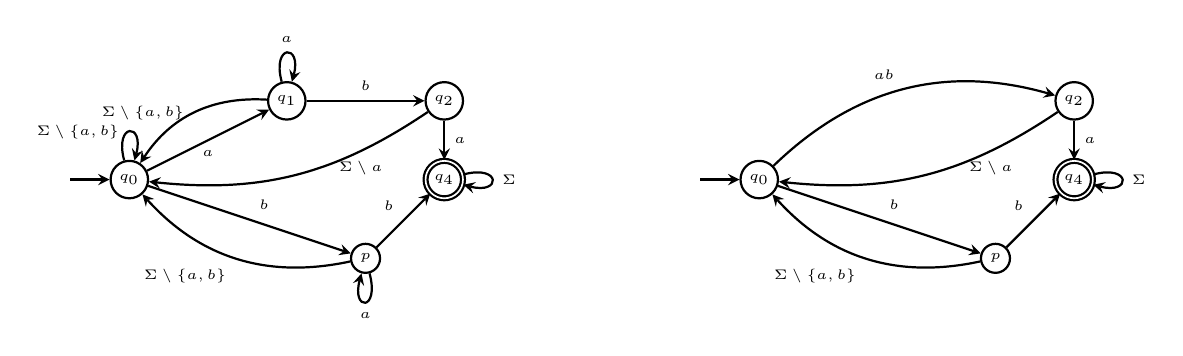
\begin{tikzpicture}[state/.style={circle, draw, thick, inner sep =
      2pt}]
    \begin{scope}[every node/.style={state}]
      \node (0) at (0,0) {\tiny $q_0$}; \node (1) at (2,1) {\tiny
        $q_1$}; \node (2) at (4,1) {\tiny $q_2$}; \node [double] (3)
      at (4, 0) {\tiny $q_4$}; \node (45) at (3,-1) {\tiny $p$};
    \end{scope}

    \begin{scope}[->,>=stealth, thick, auto]
      \draw (-0.75, 0) to (0); \draw (0) to [loop above] node [left]
      {\tiny $\Sigma \setminus \{a, b\}$} (0); \draw (0) to node
      [below] {\tiny $a$} (1); \draw (1) to [bend right=30] node
      [left] {\tiny $\Sigma \setminus \{a, b\}$} (0); \draw (1) to
      [loop above] node {\tiny $a$} (1); \draw (1) to node {\tiny $b$}
      (2); \draw (2) to [bend left=20] node [below, near start] {\tiny
        $\Sigma \setminus a$} (0); \draw (2) to node {\tiny $a$} (3);
      \draw (0) to node {\tiny $b$} (45);
      
      \draw (45) to node {\tiny $b$} (3);
 
      \draw (45) to %[near start]
      [bend left] node {\tiny $\Sigma \setminus \{a,b\}$} (0); \draw
      (45) to [loop below] node {\tiny $a$} (45); \draw (3) to [loop
      right] node {\tiny $\Sigma$} (3);
    \end{scope}

    \begin{scope}[xshift=8cm]
      \begin{scope}[every node/.style={state}]
        \node (0) at (0,0) {\tiny $q_0$}; \node (2) at (4,1) {\tiny
          $q_2$}; \node [double] (3) at (4, 0) {\tiny $q_4$}; \node
        (45) at (3,-1) {\tiny $p$};
      \end{scope}
      
      \begin{scope}[->, >=stealth, thick, auto]
        \draw (-0.75, 0) to (0);
        
        \draw (0) to [bend left] node {\tiny $ab$} (2);
        
        \draw (2) to [bend left=20] node [below, near start] {\tiny
          $\Sigma \setminus a$} (0); \draw (2) to node {\tiny $a$}
        (3); \draw (0) to node {\tiny $b$} (45);
        
        \draw (45) to node {\tiny $b$} (3);
 
        \draw (45) to 
        [bend left] node {\tiny $\Sigma \setminus \{a, b\}$}
        (0); 
        \draw (3) to [loop right] node {\tiny $\Sigma$} (3);
      \end{scope}
    \end{scope}
  \end{tikzpicture}
  \caption{DFA $M^*$ on the left and a derived DSA $\Aa^*_S$ with
    $S = \{q_0, q_2, q_4, p\}$ on the right.}
  \label{fig:dfa-m-star-dsa}
\end{figure}

\begin{figure}
  \centering
  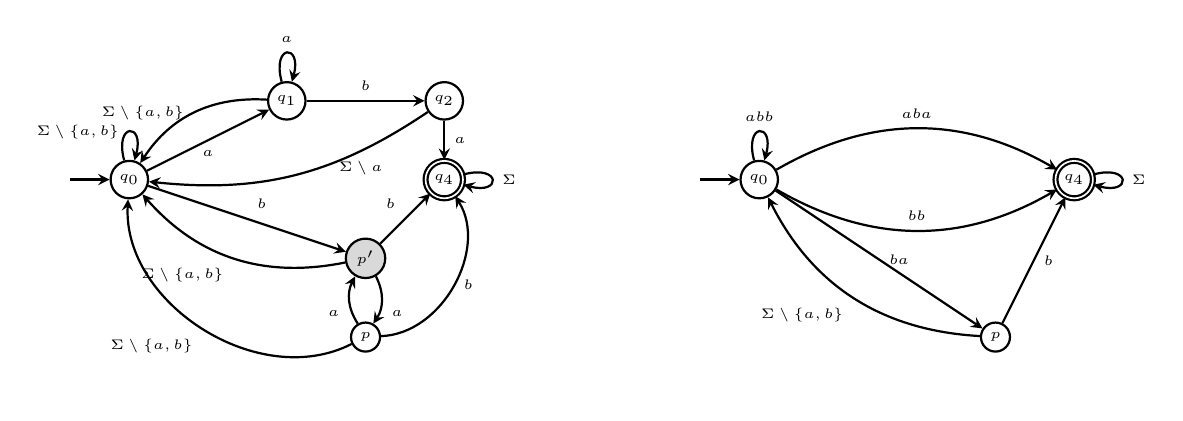
\begin{tikzpicture}[state/.style={circle, draw, thick, inner sep =
      2pt}]
    \begin{scope}[every node/.style={state}]
      \node (0) at (0,0) {\tiny $q_0$}; \node (1) at (2,1) {\tiny
        $q_1$}; \node (2) at (4,1) {\tiny $q_2$}; \node [double] (3)
      at (4, 0) {\tiny $q_4$}; \node [fill=gray!30] (4) at (3,-1)
      {\tiny $p'$}; \node (5) at (3,-2) {\tiny $p$};
    \end{scope}
    \begin{scope}[->,>=stealth, thick, auto]
      \draw (-0.75, 0) to (0); \draw (0) to [loop above] node [left]
      {\tiny $\Sigma \setminus \{a, b\}$} (0); \draw (0) to node
      [below] {\tiny $a$} (1); \draw (1) to [bend right=30] node
      [left] {\tiny $\Sigma \setminus \{a, b\}$} (0); \draw (1) to
      [loop above] node {\tiny $a$} (1); \draw (1) to node {\tiny $b$}
      (2); \draw (2) to [bend left=20] node [below, near start] {\tiny
        $\Sigma \setminus a$} (0); \draw (2) to node {\tiny $a$} (3);
      \draw (0) to node {\tiny $b$} (4); \draw (4) to [bend left] node
      {\tiny $a$} (5); \draw (5) to [bend left] node {\tiny $a$} (4);
      \draw (4) to node {\tiny $b$} (3); \draw (5) to [bend
      right=60]node [right] {\tiny $b$} (3); \draw (4)
      to 
      [bend left] node {\tiny $\Sigma \setminus \{a,b\}$} (0); \draw
      (5) to [bend left=60] node {\tiny $\Sigma \setminus \{a,b\}$}
      (0); \draw (3) to [loop right] node {\tiny $\Sigma$} (3);
    \end{scope}

    \begin{scope}[xshift=8cm]
      \begin{scope}[every node/.style={state}]
        \node (0) at (0,0) {\tiny $q_0$}; \node [double] (3) at (4, 0)
        {\tiny $q_4$}; \node (5) at (3,-2) {\tiny $p$};
      \end{scope}
      \begin{scope}[->, >=stealth, thick, auto]
        \draw (-0.75, 0) to (0); \draw (0) to [bend left] node {\tiny
          $aba$} (3); \draw (0) to [bend right] node {\tiny $bb$} (3);
        \draw (0) to node [right] {\tiny $ba$} (5); \draw (5) to node
        [right] {\tiny $%ab,
          b$} (3); \draw (5) to [bend left] node {\tiny
          $\Sigma\setminus \{ a, b\}$} (0); \draw (0) to [loop above]
        node {\tiny $abb$} (0); \draw (3) to [loop right] node {\tiny
          $\Sigma$} (3);
      \end{scope}
    \end{scope}
  \end{tikzpicture}
  \caption{DFA $M^{**}$ on the left and a derived DSA $\Aa^{**}_S$
    with $S = \{q_0, q_2, q_4, p\}$ on the right.}
  \label{fig:m-star-star}
\end{figure}

Figure~\ref{fig:dfa-m-star-dsa} shows a DFA $M^*$. Observe that $M^*$
is minimal: every pair of states has a distinguishing suffix. Let us
now look at DSAs that can be derived from $M^*$. Firstly, any
suffix-tracking set on $M^*$ would contain $q_0, q_4$ (since they are
initial and accepting states). If $p$ is not picked, the transition
$p \xra{a} p$ is not suffix-compatible. Therefore, $p$ should belong
to the selected set. If $p$ is picked, and $q_2$ not picked, then the
set is not well-formed (see Definition~\ref{def:well-formed-set}): the
simple word $b$ from $q_0$ to $p$ is a suffix of the simple word $ab$
to $q_2$. Therefore, any suffix-tracking set should contain the $4$
states $q_0, p, q_2, q_4$. This set $S = \{q_0, p, q_2, q_4\}$ is
indeed suffix-tracking, and the DSA derived using $S$ is shown in the
right of Figure~\ref{fig:dfa-m-star-dsa}. The only other
suffix-tracking set is the set $S'$ of all states. The DSA derived
using $S'$ will have state $q_1$ in addition, and the transitions
$\Sigma \setminus \{a, b\}$. If $\Sigma$ is sufficiently large, this
DSA would have total size bigger than $\Aa^*_S$ (Note: $\Sigma$ can be any alphabet containing $a$ and $b$, so we can increase its size arbitrarily to blow up the DSA). We deduce $\Aa^*_S$
to be the smallest DSA that can be derived from $M^*$.

Figure~\ref{fig:m-star-star} shows DFA $M^{**}$ which is obtained from
$M^*$ by duplicating state $p$ to create a new state $p'$, which is
equivalent to $p$. So $M^{**}$ is language equivalent to $M^*$, but it
is not minimal. Here, if we choose $p$ in a suffix-tracking set, the
simple word to $p$ is $ba$, which is not a suffix of $ab$ (the simple
word to $q_2$). Hence, we are not required to add $q_2$ into the
set. Notice that $S = \{q_0, p, q_4\}$ is indeed a suffix-tracking set
in $M^{**}$. The derived DSA $\Aa^{**}_S$ is shown in the right of the
figure. The ``heavy'' transition on $\Sigma \setminus a$
disappears. There are some extra transitions, like $q_0 \xra{bb} q_4$,
but if $\Sigma$ is large enough, the size of $\Aa^{**}_S$ will be
smaller than $\Aa^*_S$. This shows that starting from a big DFA helps
deriving a smaller DSA, and in particular, the canonical DFA of a
regular language may not derive a minimal DSA for the language.



\section{Complexity of minimization}
\label{sec:complexity}

The goal of this section is to prove the following theorem.

\begin{theorem}
  \label{thm:np-complete}
  Given a DFA $M$ and positive integer $k$, deciding whether there
  exists a DSA of total size $\le k$ language equivalent to $M$ is
  NP-complete.
\end{theorem}

If $k$ is bigger than the size of the DFA $M$, then the answer is
trivial. Therefore, let us assume that $k$ is smaller than the DFA
size. For the $\NP$ upper bound, we guess a DSA of total size $k$,
compute its tracking DFA in time $\mathcal{O}(k \cdot |\Sigma|)$ and
check for its language equivalence with the given DFA $M$. This can be
done in polynomial-time by minimizing both the DFA and checking for
isomorphism.

The rest of the section is devoted to proving the lower bound.  We
provide a reduction from the minimum vertex cover problem which is a
well-known $\NP$-complete problem~\cite{DBLP:conf/coco/Karp72}. A
vertex cover of an undirected graph $G = (V, E)$ is a subset
$S \subseteq V$ of vertices, such that for every edge $e \in E$, at
least one of its end points is in $S$. The decision problem takes a
graph $G$ and a number $k' \ge 1$ as input and asks whether there is a
vertex cover of $G$ with size at most $k'$. Using the graph $G$, we
will construct a DFA $M_G$ over an alphabet $\Sigma_G$. We then show
that $G$ has a vertex cover of size $\le k'$ iff $M_G$ has an
equivalent DSA with total size $\le k$ where
$k = (k'+2)\times 2\theta + (2 \theta - 1)$. Here, $\theta$ is a
sufficiently large polynomial in $|V|, |E|$ which we will explain
later. 

  \begin{figure}
    \centering
    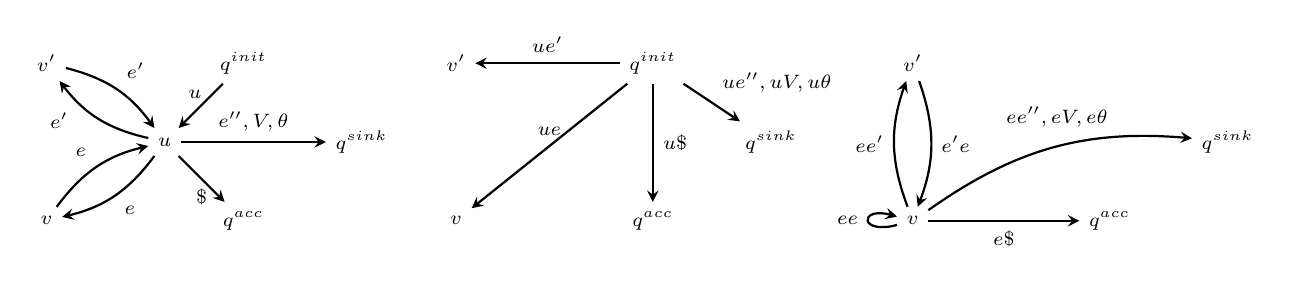
\begin{tikzpicture}
      \begin{scope}
        \node (u) at (0,0) {\scriptsize $u$}; \node (v) at (-1.5, -1)
        {\scriptsize $v$}; \node (init) at (1, 1) {\scriptsize
          $q^{init}$}; \node (acc) at (1, -1) {\scriptsize $q^{acc}$};
        \node (sink) at (2.5, 0) {\scriptsize $q^{sink}$}; \node (v')
        at (-1.5, 1) {\scriptsize $v'$};
      \end{scope}
      \begin{scope}[->,>=stealth, thick, auto]
        \draw (v) to [bend left = 20] node {\scriptsize $e$} (u);
        \draw (u) to [bend left = 20] node {\scriptsize $e$} (v);
        \draw (init) to node [left, near start] {\scriptsize $u$} (u);
        \draw (u) to node {\scriptsize $e'', V, \theta$} (sink); \draw
        (u) to node [below] {\scriptsize $\$$} (acc);

        \draw (v') to [bend left=20] node {\scriptsize
          $e'$} (u); \draw (u) to [bend left=20] node [near end]
        {\scriptsize $e'$} (v');
      \end{scope}

      \begin{scope}[xshift=5.2cm]
        \begin{scope}
          \node (v) at (-1.5, -1) {\scriptsize $v$}; \node (init) at
          (1, 1) {\scriptsize $q^{init}$}; \node (acc) at (1, -1)
          {\scriptsize $q^{acc}$}; \node (sink) at (2.5, 0)
          {\scriptsize $q^{sink}$}; \node (v') at (-1.5, 1)
          {\scriptsize $v'$};
        \end{scope}
       
      \begin{scope}[->,>=stealth, thick, auto]
        \draw (init) to node [above] {\scriptsize $ue$} (v); \draw
        (init) to node [above] {\scriptsize $ue'$} (v'); \draw (init)
        to node {\scriptsize $u \$$} (acc); \draw (init) to node
        {\scriptsize $ue'', uV, u\theta$} (sink);
      \end{scope}
    \end{scope}

    \begin{scope}[xshift=11cm]
      \node (v) at (-1.5, -1) {\scriptsize $v$};
      \node (acc) at (1, -1) {\scriptsize
        $q^{acc}$}; \node (sink) at (2.5, 0) {\scriptsize
        $q^{sink}$}; \node (v') at (-1.5, 1) {\scriptsize $v'$};
    \end{scope}

      \begin{scope}[->,>=stealth, thick, auto]
        \draw (v) to [bend left = 20] node {\scriptsize $ee'$} (v');
        \draw (v') to [bend left=20] node {\scriptsize $e'e$} (v);
        \draw (v) to node [below] {\scriptsize $e\$$} (acc); \draw (v)
        to [bend left=20] node [near end] {\scriptsize $ee'', eV,
          e\theta$} (sink); \draw (v) to [loop left] node {\scriptsize
          $ee$} (v);
      \end{scope}
    \end{tikzpicture}
    \caption{Left: Illustration of the neighbourhood of state
      $u$ in the DFA
      $M_G$. Middle, Right: Transitions induced from
      $q^{init}$ and $v$, on removing $u$.}
    \label{fig:complexity-mg}
  \end{figure}

  The alphabet $\Sigma_G$ is given by $V \cup E \cup \{ \$\} \cup
  D$ where $D = \{1,2, \dots, \theta\}$. States of $M_G$ are $V \cup
  \{q^{init}, q^{sink},
  q^{acc}\}$. For simplicity, we use the same notation for
  $v$ as a vertex in $G$, $v$ as a letter in $\Sigma_G$ and
  $v$ as a state of $M_G$. The actual role of
  $v$ will be clear from the context. For every edge $e = (u,
  v)$, there are two transitions in the automaton: $u \xra{e}
  v$ and $v \xra{e} u$. For every $v \in
  V$, there are transitions $q^{init} \xra{v} v$ and $v \xra{\$}
  q^{acc}$. This automaton can be completed by adding all missing
  transitions to the sink state
  $q^{sink}$. Figure~\ref{fig:complexity-mg} (left) illustrates the
  neighbourhood of a state $u$. The notation
  $e''$ stands for any edge that is not incident on
  $u$; there is one transition for every such
  $e''$. Initial and accepting states are respectively
  $q^{init}$ and $q^{acc}$.
  Let
  $L_G(u)$ be the set of words that have an accepting run in
  $M_G$ starting from
  $u$ as the initial state. 
  If $u \neq v$, $L_G(u) = L_G(v)$ implies
  $(u,v)$ is an edge and there are no other edges outgoing either from
  $u$ or
  $v$. To avoid this corner case, we restrict the vertex cover problem
  to connected graphs of 3 or more vertices. Then we have
  $M_G$ to be a minimal DFA, with no two states equivalent. Here are
  two main ideas.
  

  \emph{Suppressing a state.} Suppose state $u$ of $M_G$
  is suppressed (i.e. $u$ is not in a suffix-tracking
  set). In Figure~\ref{fig:complexity-mg}, we show
  the induced transitions from $q^{init}$ and a vertex $v$. However,
  some of them will be useless transitions: most importantly, the set
  of transitions $q^{init} \xra{u1, u2, \dots, u\theta} q^{sink}$ will
  be useless bigger-suffix-transitions due to
  $q^{init} \xra{1, 2, \dots, \theta} q^{sink}$. Similarly,
  $v \xra{e1, e2, \dots, e\theta} q^{sink}$ will be removed. There are
  some more useless bigger-suffix-transitions, like
  $v \xra{e e''} q^{sink}$ for some $e''$ that is not incident on $v$
  and $u$. So from each $v$, at most $2 |E|$ transitions are
  added. But crucially, after removing
  useless transitions, the $\theta$ transitions from $u$
  no longer appear. If we choose $\theta$ large enough to compensate
  for the other transitions, we get an overall reduction in size by
  suppressing states.


 

  \emph{Two states connected by an edge cannot both be suppressed.}  Suppose $e = (u, v)$ is an edge. If $S$ is a set where
  $u, v \notin S$, then the transition $v \xra{e} u$ is not
  suffix-compatible: the simple word $ue$ from $q^{init}$ to $v$, when
  extended with $e$ gives the word $uee$; no suffix of $uee$ is a
  simple word from $q^{init}$ to $u$. We deduce that
  suffix-tracking sets in $M_G$ correspond to a vertex cover in $G$,
  and vice-versa.

  These two observations lead to a translation from minimum vertex
  cover to suffix-tracking sets with least number of states. Due to
  our choice of $\theta$, DSAs with smallest (total) size are indeed
  obtained from suffix-tracking sets with the least number of states. 
Let $k = (k' + 2) \times 2 \theta + (2 \theta - 1)$. Below, we elaborate these ideas in more detail and present the proof of the reduction.



\subparagraph*{Vertex cover $\le k'$ implies DSA $\le k$.}
Assume there is a vertex cover $\{v_1,
  \dots, v_p \}$ in $G$ with $p \le k'$. Let $S$ be the set of states in $M_G$ corresponding to $\{v_1,
  \dots, v_p \}$. Observe that $S \cup \{q^{init},q^{sink},q^{acc}\}$ is a suffix-tracking set; every transition is trivially suffix-compatible ($\forall q\xra{a}u, q\in S \text{ or } u\in S $). Well-formedness holds because $\forall p,q \in S, \a \in \spath{p}{q}{S}$ we have $|\a| \le 2$; this means $\forall q' \notin S, \beta \in \spath{p}{q'}{S}$, we have
  $\a \not \sfx \beta$ (since $|\beta|=1$). Hence the derived DSA will be equivalent to $M$.

  The derived DSA has $p + 3$ states, and transitions $q \xra{1, 2, \dots,
\theta} q^{sink}$ from each except for the $q^{sink}$ state. The
transitions on $q^{sink}$ are removable, and hence will be absent. All of this adds $(p+2) \times 2 \theta$ to the total size (edges +
label lengths). Apart from these, there are transitions with
labels of length at most $2$, over the alphabet $V \cup E \cup \$$. From each vertex, $v$, there are $|V|$ transitions to $q^{sink}$, one transition to $q^{acc}$ and at most $2|E|$ transitions to other states or $q^{sink}$. We
can choose a large enough $\theta$ (say $(|V| + |E|)^4$), so that the size of
these extra transitions is at most $2 \theta - 1$. 
  Hence, total size is $\le (p + 2) \times 2 \theta + (2 \theta - 1)$.

By assumption, we have $p \le k'$. Therefore, the size of the DSA 
is $\le (k' + 2) \times 2 \theta + (2 \theta - 1)%$, which is precisely $
=k$.

 

  \subparagraph*{DSA $\le k$ implies vertex cover $\le k'$.}

  Let $\Aa$ be a DSA with size $\le k$. It may not be derived from $M_G$. However, by Proposition~\ref{prop:dsa-derivable-from-tracking-dfa} we know $\Aa$ is derived from a DFA $M$, the tracking DFA for $\Aa$. Moreover since $M_G$ is the minimal DFA, we know that $M$ will be a \emph{refinement} of $M_G$ (see Section~\ref{sec:preliminaries} for definition).


  
  Let us consider a pair of states $u$ and $v$ from $M_G$, such that the vertices $u,v \in G$ have an edge between them labeled $e$. The DFA $M$ will have two sets of states $u_1,u_2,\dots,u_i$ and $v_1,v_2,\dots,v_j$ that are language-equivalent to $u$ and $v$ respectively. Its initial state must have a transition on $v$ to one of $v_1,v_2,\dots,v_j$. Without loss of generality, let it be to $v_1$. Each of $v_1,v_2,\dots,v_j$ must have a transition on $e$ to one of $u_1,u_2,\dots,u_i$ (for equivalence with $M_G$) and vice-versa. Consider the run from the initial state on $ve^{i+j+1}$. At least one of the states among $u_1,u_2,\dots,u_i, v_1,v_2,\dots,v_j$ must be visited twice; consider the first such instance. The transition on $e$ that re-visits a state cannot be suffix-compatible w.r.t a set $S$, if none of these states are in $S$. For it to be suffix-compatible, the string $ve^k.e$ (from initial state to the first repeated state) must have its longest simple-word suffix go the same state. Since $ve^k.e$ is not simple by itself, its longest suffix must consist entirely of $e$'s. But on any string of $e$'s, the initial state moves only to the sink state(s) and not to any of $u_1,u_2,\dots,u_i, v_1,v_2,\dots,v_j$. Hence any suffix-tracking set must contain at least one of these states, which maps to at least one of $u$ or $v$ in $G$. Every suffix-tracking set of $M$ therefore maps to a vertex cover $\{v_1, v_2, \dots, v_p\}$.
  

  
  Now we show that the size of this vertex cover is $\le k'$.
Each of the states picked in the suffix-tracking set will contribute to atleast $2 \theta$ in the total size, due to the $\theta$ transitions. We will also have these $\theta$ transitions from the initial and accepting states. Therefore, the total size is $(p + 2) \times 2 \theta + y$ for some $y > 0$. Hence $(p + 2) \times 2 \theta \le k$. This implies $p \le k'$: otherwise we will have $p \ge k'+1$, and hence $(p + 2) \times 2 \theta \ge (k' + 1 + 2) \times 2 \theta = (k' + 2) \times 2 \theta + 2 \theta > k$, a contradiction.   


  

%%% Local Variables:
%%% mode: latex
%%% TeX-master: "dsa-main"
%%% End:


\section{Strongly Deterministic Suffix-reading Automata (sDSA)}
\label{sec:strong}

As we saw in Section~\ref{sec:minim-some-observ}, the minimal DFA of a
regular language may not derive a minimal DSA for the language (Figures~\ref{fig:dfa-m-star-dsa} and Figure~\ref{fig:m-star-star}). While this is true for the general case, under a restricted definition of DSA we can show the minimal DFA to derive a minimal (restricted) DSA. The plan for this section is as follows:

\begin{description}
\item[Section~\ref{sec:sDSA-syntax}] We first define a class of DSAs with a restricted syntax and call them \emph{strongly deterministic} suffix-reading automata or \emph{strong DSAs} (Definition~\ref{def:str-suff-reading-aut}) and give examples of DSAs that fall under this stronger class.
\item[Section~\ref{sec:sDSA-minimality}]  In the second part, we prove that every minimal strong DSA can be derived from the canonical DFA using the derivation procedure of Section~\ref{sec:suffix-tracking-sets}.
\end{description}

This section is inspired by a question that was left open in the earlier version of this work~\cite{DBLP:journals/corr/abs-2410-22761}: when does the smallest DSA derived from the canonical DFA correspond to a minimal DSA? Although we do not provide an answer to this question, we now understand that when we suitably restrict the DSA syntax, the derivation procedure indeed is able to generate a minimal automaton in the restricted class, starting from the canonical DFA. This provides new insights about the derivation procedure. Moreover, as we will see, many DSAs discussed in this paper are already strong. We also provide a real-life-inspired example of a strong DSA. So, overall, this section sends the message that there are specifications that can be encoded naturally as strong DSAs, and we have a method to generate minimal strong DSAs. 

\subsection{Syntax of strong DSAs}
\label{sec:sDSA-syntax}

We start with a formal description of the syntax of strong DSAs. The examples that follow aim to give an explanation of this definition. In this definition, we say $\alpha'$ is a non-empty prefix of a word $\alpha$ when $\alpha' \neq \epsilon$ and $\alpha' \prfx \alpha$. 

\begin{definition}[sDSA]\label{def:str-suff-reading-aut}
(Strongly Deterministic Suffix-reading Automata). A DSA $\Aa = (Q, \Sigma, q_{init}, \Delta, F)$ is said to be strongly deterministic if for every state $q \in Q$, for every $\a, \beta \in \out (q)$, and for all non-empty prefixes $\a' \prfx \a$ and all non-empty proper prefixes $\beta' \pprfx \beta$, we have $\a' \not \sfx \beta'$ : no prefix of $\a$ is a factor of $\beta$.
\end{definition}

For instance, the DSA in Figure~\ref{fig:if-else} is not an sDSA: at state $s_1$ we have $\out(s_1) = \{ \text{\texttt{if}}, \text{\texttt{endif}}\}$, and the letter \texttt{i} (which is a prefix of \texttt{if}) appears in \texttt{endif} as a suffix  of \texttt{endi}. The DSAs in Figures~\ref{fig:example-aab} and \ref{fig:example-ab-bb} are strong DSAs: it is easy to verify this for $\Aa_2$ and $\Aa_3$; for $\Aa_4$, we provide an explanation. We have $\out(q_0) = \{ab , ba\}$; let $\alpha = ab$ and $\beta= ba$. The non-empty prefixes of $\alpha$ are $a$ and $ab$. The only non-empty proper prefix of $\beta$ is $b$. Notice that neither $a$ nor $ab$ is a suffix of $b$. The same exercise can be repeated with $\alpha = ba$ and $\beta = ab$. We conclude that $\Aa_4$ is an sDSA. Note that any DFA is an sDSA, as the labels of each outgoing transition at a state are distinct letters (and a DFA is a valid DSA). A slightly modified version of the DSA in Figure~\ref{fig:if-else} gives us an example of an sDSA. In Figure~\ref{fig:if-else-no-nest} we have a DSA for out-of-context \texttt{else} statements, where we allow nested \texttt{if}, but a single \texttt{endif} appearing later corresponds to all the open \texttt{if} so far. A context would therefore be the part between the first \texttt{if} and the last \texttt{endif}. If the specification additionally requires to disallow nested \texttt{if}, then it can be modeled by the intersection of the sDSA of Figure~\ref{fig:if-else-no-nest} and another automaton that rejects words with two \texttt{if} with no \texttt{endif} in between.

\begin{figure}[t]
  \centering
  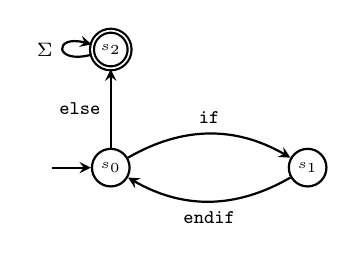
\begin{tikzpicture}[state/.style={circle, draw, thick, inner sep =
      2pt}]
    \begin{scope}[every node/.style={state}]
      \node (0) at (0,0) {\tiny $s_0$}; \node (1) at (2.5, 0) {\tiny
        $s_1$}; \node [double] (2) at (0, 1.5) {\tiny $s_2$}; 
    \end{scope}
    \begin{scope}[->, >=stealth, thick, auto]
      \draw (-0.75, 0) to (0); \draw (0) to node {\scriptsize
        $\mathtt{else}$ } (2); \draw (0) to [bend left=30] node
      {\scriptsize $\mathtt{if}$} (1); \draw (1) to [bend left=30]
      node {\scriptsize $\mathtt{endif}$} (0); \draw (2) to [loop
      left] node {\scriptsize $\Sigma$} (2); 
    \end{scope}
  \end{tikzpicture}
  \caption{sDSA for out-of-context \texttt{else}, without nested if statements}
  \label{fig:if-else-no-nest}
\end{figure}

We describe another example of a strong DSA, motivated by a real-life situation. It is a simplified specification of an automotive
application: ``when the alarm is off, and the panic switch is pressed
twice within one clock cycle, go to an error state''. The DFA in
Figure~\ref{fig:automotive-eg} models this. States $q_0$ and $q_1$
represent the alarm being off and on respectively. State $q_3$ is the
error state. The DFA toggles between off and on states on receiving
Signal $s$.  Signal $t$ denotes a ``tick'' marking the separation of
clock cycles, and $p$ denotes the pressing of the panic switch. The
sDSA for this specification is given on the right of
Figure~\ref{fig:automotive-eg}. At state $q_0$, the automaton keeps
receiving signals until either an $s$ or a sequence $pp$ is seen. If
$s$ is seen first, the automaton moves to $q_1$, otherwise it moves to
$q_3$. The move on $q_0 \xra{pp} q_3$ happens on words over
$\{t, p, s\}$ that end with $pp$, and contain neither an $s$ nor a
previous occurrence of $pp$.  This expresses that the panic switch was
pressed twice, within one clock cycle (as no $t$ occurred), while the
alarm was still off. Here, the sDSA provides a smaller, and arguably, a
more readable representation than the DFA.

\begin{figure}[t]
  \centering
  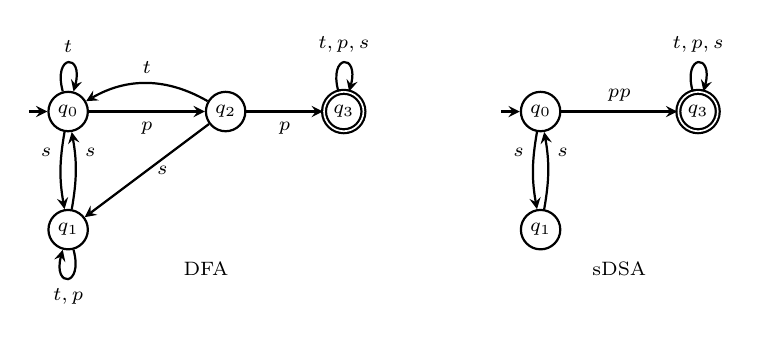
\begin{tikzpicture}[state/.style={draw, thick, circle, inner
      sep=2pt}]
    \begin{scope}[every node/.style={state}]
      \node (0) at (0,0) {\scriptsize $q_0$}; \node (1) at (0,-1.5)
      {\scriptsize $q_1$}; \node (2) at (2,0) {\scriptsize $q_2$};
      \node [double] (3) at (3.5,0) {\scriptsize $q_3$};
    \end{scope}
    \begin{scope}[->, thick, >=stealth, auto]
      \draw (-0.5, 0) to (0); \draw (0) to [loop above] node
      {\scriptsize $t$} (0); \draw (0) to [bend right=10] node [left,
      near start] {\scriptsize $s$} (1); \draw (1) to [bend right=10]
      node [right, near end] {\scriptsize $s$} (0); \draw (0) to node
      [below] {\scriptsize $p$} (2); \draw (2) to [bend right=30] node
      [above] {\scriptsize $t$} (0); \draw (2) to node [right]
      {\scriptsize $s$} (1); \draw (2) to node [below] {\scriptsize
        $p$} (3); \draw (3) to [loop above] node {\scriptsize
        $t, p, s$} (3); \draw (1) to [loop below] node {\scriptsize
        $t, p$} (1);
    \end{scope}
    \node at (1.75, -2) {\scriptsize DFA};

    \begin{scope}[xshift=6cm]
      \begin{scope}[every node/.style={state}]
        \node (0) at (0,0) {\scriptsize $q_0$}; \node (1) at (0,-1.5)
        {\scriptsize $q_1$}; \node [double] (3) at (2,0) {\scriptsize
          $q_3$};
      \end{scope}
      \begin{scope}[->, thick, >=stealth, auto]
        \draw (-0.5, 0) to (0); \draw (0) to node {\scriptsize $pp$}
        (3); \draw (0) to [bend right=10] node [left, near start]
        {\scriptsize $s$} (1); \draw (1) to [bend right=10] node
        [right, near end] {\scriptsize $s$} (0); \draw (3) to [loop
        above] node {\scriptsize $t, p, s$} (3);
      \end{scope}
      \node at (1, -2) {\scriptsize sDSA};
    \end{scope}
  \end{tikzpicture}
  \caption{A simplified specification of an automotive application}
  \label{fig:automotive-eg}
\end{figure}


However sDSA may not always provide as succinct a representation as DSA. We see in Figure \ref{fig:dsa-smaller-sdsa-eg}, an example of a DSA on the left and an equivalent sDSA on the right. It is the DSA from Figure \ref{fig:dsa-to-dfa-eg} again, with the corresponding sDSA shown. The DSA itself is not a valid sDSA, since $ba$ is a prefix of $baaa$ and a factor of $abaa$ (also $a$ is prefix of $abaa$ and a factor of $baaa$). Intuitively, to construct an sDSA, we need to break the transitions after $ab$ and $ba$ and introduce new states. This continues to happen on the next transitions from these new states, resulting in the sDSA shown.

\begin{figure}
  \centering
  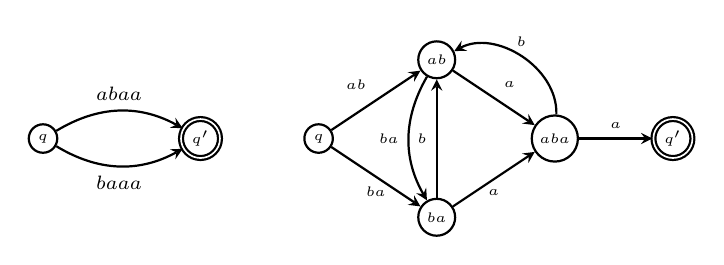
\begin{tikzpicture}[state/.style={circle, draw, thick, inner sep =
      2pt}]
    \begin{scope}[every node/.style={state}]
      \node (0) at (0,0) {\tiny $q$}; \node [double] (1) at (2,0)
      {\tiny $q'$};
    \end{scope}
    \begin{scope}[->, >=stealth, thick, auto]
      \draw (0) to [bend left=30] node {\scriptsize $abaa$} (1); \draw
      (0) to [bend right=30] node [below] {\scriptsize $baaa$} (1);
    \end{scope}

    \begin{scope}[xshift=3.5cm]
      \begin{scope}[every node/.style={state}]
        \node (0) at (0,0) {\tiny $q$}; %\node (a) at (1,1) {\tiny $a$}; \node (b) at (1,-1) {\tiny $b$}; 
        \node (ab) at (1.5, 1) {\tiny $ab$}; 
        \node (ba) at (1.5,-1) {\tiny $ba$}; 
        \node (aba) at (3, 0) {\tiny $aba$}; 
        %\node (baa) at (3,-1) {\tiny $baa$};
        \node [double] (1) at (4.5, 0) {\tiny $q'$};
      
      \end{scope}
      \begin{scope}[->,>=stealth, thick, auto]
        \draw (0) to node {\tiny $ab$} (ab); 
        \draw (0) to node [below] {\tiny $ba$} (ba); 
        %\draw (a) to node {\tiny $b$} (ab); \draw (b) to node [below] {\tiny $a$} (ba); 
        \draw (ab) to node {\tiny $a$} (aba); 
        \draw (ba) to node [below] {\tiny $a$} (aba); 
        \draw (aba) to node {\tiny $a$} (1); 
        %\draw (baa) to node [below] {\tiny $a$} (1); 
        %\draw (b) to [loop below] node {\tiny $b$} (0); \draw (a) to [loop above] node {\tiny $a$} (a); 
        \draw (ba) to node {\tiny $b$} (ab); 
        %\draw (baa) to node {\tiny $b$} (ab); 
        \draw (ab) to [bend right=30] node [left] {\tiny $ba$} (ba); 
        \draw (aba) to [bend right=60] node [above] {\tiny $b$} (ab);
      \end{scope}

    \end{scope}

  \end{tikzpicture}
  \caption{A DSA on the left, and the corresponding (larger) sDSA}
  \label{fig:dsa-smaller-sdsa-eg}
\end{figure}

\subsection{Minimality for strong DSAs}
\label{sec:sDSA-minimality}

 We state some preliminary lemmas, leading up to the main result that any minimal sDSA is derived from a minimal DFA. The next lemma is generic and holds for all DSAs, which are not necessarily strong. We start with some notation. 

 For a state $q$ of a DFA $M$, we define $L^M(q)$ to be the words accepted by $M$ starting from $q$ and call it the \emph{residual language} of the state. Similarly, for a DSA $\Aa$ and a state $q$ of $\Aa$, we can define the residual language $L^\Aa(q)$.
 We say that two states $p, q$ of a DFA/DSA are \emph{equivalent} if their residual languages are equal. In the setting of DFAs, we know that in the canonical (minimal-state) automaton, no two states are equivalent. The next lemma establishes this property even in the DSA setting.

\begin{lemma}\label{lem:minimal-dsa-no-equivalent-states}
No two states of a minimal DSA can be equivalent.
\end{lemma}

\begin{proof}
  Let $\Aa$ be a minimal DSA. Suppose 
  $L^\Aa(p) = L^\Aa(q), p \ne q$. We will
  now construct a DSA $\Aa'$ with smaller size
  than $\Aa$. This will be a contradiction. To get $\Aa'$, we will
  re-orient all transitions going to $q$ to now point towards $p$:
  remove each 
  transition $(r, \a, q)$ and add the transition $(r, \a, p)$; then
  remove $q$ and other unreachable states after this
  transformation. Since $L^\Aa(p) = L^\Aa(q)$, this construction
  preserves the language. For all the states $r$ that remain in $\Aa'$ we
  still have the same $\out(r)$ as in $\Aa$. Finally we need to argue that $|\Aa'| <
  |\Aa|$. This is easy to see since $q$ has been removed from $\Aa$,
  and there are no new additions to $\Aa'$.
\end{proof}

   
Now we come to properties specific to sDSAs. The key idea is to consider the tracking DFA (Definition~\ref{def:tracking-dfa} and Figure~\ref{fig:dsa-to-dfa-eg}) and investigate equivalence between states in this tracking DFA. 

\begin{lemma}\label{lem:sdsa-equivalent-states}
For any minimal sDSA $\Aa$, its tracking DFA $M_\Aa$ cannot have a `DSA state' equivalent to any other state, i.e. if $(p,\a),(q,\beta)$ are states of $M_\Aa$ and also equivalent, then we have both $\a\ne\e$ and $\beta\ne\e$.
\end{lemma}

\begin{proof}
From Lemma~\ref{lem:minimal-dsa-no-equivalent-states}, we know that no two states of any minimal DSA can be equivalent. So it is not possible to have any distinct $(p,\e),(q,\e) \in M_\Aa$ to be equivalent. Suppose $L^{M_\Aa}(p, \e) = L^{M_\Aa}(q, \beta)$ for some $\beta \ne \e$ (and $q$ could be $p$ as well). We will construct a smaller sDSA $\Aa'$. 

Consider state $q$ of $\Aa$. Due to the presence of state $(q, \beta)$ in $M_\Aa$, there exists some outgoing label of the form $\beta\a$ from $q$ in $\Aa$: that is, $\beta\a \in \out(q)$ for some $\a$ with $|\a| \ge 1$. Let the corresponding transition be $q \xra{\beta\a} r$. To get $\Aa'$ : remove this transition $q\xra{\beta\a}r$ and add the transition $q\xra{\beta}p$. Clearly $\Aa'$ is smaller than $\Aa$, since total size is reduced by $|\a|$. Language accepted is the same. $\Aa'$ is also an sDSA since the only change is replacing $\beta\a$ with $\beta$ in $\out(q)$: any string in $\outp(q)$ that is a factor of $\beta$ would also be a factor of $\beta\a$, and any prefix of $\beta$ is also a prefix of $\beta\a$. This contradicts the assumption that $\Aa$ was a minimal sDSA, thus proving the lemma.
\end{proof}

We remark that the above proof does not work for general DSAs. Consider the transition $q \xra{\beta \alpha} r$ that was removed, and modified to $q \xra{\beta} p$. There could be another transition $q \xra{\beta \alpha'} r'$ in the DSA --- this violates the strong DSA property since $\beta \alpha$ and $\beta \alpha'$ are outgoing labels, and the prefix $\beta$ of the former appears as a suffix of the latter. On seeing the word $\beta \alpha'$ from $q$, the original DSA moves to $r'$. However, in the new DSA, as soon as $\alpha$ is seen the state changes to $p$. This can modify the language. Such a situation does not happen in an sDSA due to the restriction on the outgoing labels. We now prove the main result of this section.

\begin{theorem}
Every minimal sDSA for a language $L$ can be derived from the canonical DFA for $L$.
\end{theorem}


\begin{proof}

  Let $\Aa = (Q^\Aa, \Sigma, \Delta^\Aa, F^\Aa)$ be an arbitrary minimal sDSA.
Any minimal sDSA is well-formed and has no redundant transitions. Hence $\Aa$ can be derived from its tracking DFA $M_\Aa$, thanks to Proposition~\ref{prop:dsa-derivable-from-tracking-dfa}. If the tracking DFA $M_\Aa$ is canonical, we are done. Otherwise, there are distinct states of $M_\Aa$ that are equivalent.  From Lemma~\ref{lem:sdsa-equivalent-states}, we know that a state $(q, \epsilon)$ of $M_\Aa$ cannot be equivalent to any other state. Therefore,  two equivalent states are of the form $(p, \alpha)$ and $(q, \beta)$, with $\alpha$ and $\beta$ both non-empty. We will merge such equivalent states together to build the minimal automaton and make use of this specific structure to show that $\Aa$ can be derived from the minimized DFA. For the proof, we will show the following steps.
\begin{enumerate}
\item Suppose a state $(q, \alpha)$ is equivalent to $(q, \beta)$ (with the same $q$), then $\alpha \not \prfx \beta$ (i.e. the two states cannot be `tracking' the same $\Aa$-transition out of $q$).
\item Build a DFA $M'_\Aa$ by quotienting equivalent states of $M_\Aa$, with $[q]$ representing the equivalence class of $q$. The resulting automaton $M'_\Aa$ is the canonical DFA. We use (1) to show that every simple path from a state $(q, \epsilon)$ to $(q, \beta)$ is preserved in the quotiented automaton $M'_\Aa$, from $[(q, \epsilon)]$ to $[(q, \beta)]$.
\item From (2), we show that the set of states $S' := \{ [(q, \epsilon)] \mid q \in Q^\Aa\}$ forms a suffix-tracking set. The DSA derived using $S'$ turns out to be $\Aa$, proving that $\Aa$ can be derived from the canonical DFA.
\end{enumerate}

\paragraph*{Step 1.} If two states $(q,\a),(q,\beta) \in M_\Aa$ are equivalent, then $\a\nprfx\beta$ (i.e. the two states are not `tracking' the same $\Aa$-transition). In other words, two states in the tracking DFA that lie on the same path corresponding to a given DSA transition, cannot be equivalent. Suppose $\a\prfx\beta$. We know that $\beta\in\outp(q)$, so there is a string $\gamma$ such that $\beta\gamma\in\out(q)$ i.e. reading $\gamma$ from $(q,\beta)$ leads to a `DSA state', say $(q',\e)$. Let $s$ be the state reached on reading $\gamma$ from $(q, \alpha)$. Since $(q, \alpha)$ and $(q, \beta)$ are equivalent, the state $s$ will be equivalent to $(q', \e)$. From Lemma~\ref{lem:sdsa-equivalent-states}, this means $s = (q', \e)$. This gives transition labels $\a\gamma$ (induced by the simple path just discussed) and $\beta\gamma$ from $q$ in $\Aa$, with $\a\prfx\beta$, contradicting the fact that $\Aa$ was an sDSA. Hence we must have $\a\nprfx\beta$.

\paragraph*{Step 2.} For two states $s, s'$ of $M_\Aa$, define $s \equiv_{M_\Aa} s'$ if $L^{M_\Aa}(s) = L^{M_\Aa}(s')$. We denote the equivalence class of $s$ by $[s]$. From Lemma~\ref{lem:sdsa-equivalent-states}, $[(q, \epsilon)] = \{ (q, \epsilon)\}$. Consider a quotient DFA $M'_\Aa$ based on this equivalence. States are the equivalence classes of $\equiv_{M_\Aa}, \{ [s] \mid s \in M_\Aa \}$. 
The initial state is $[(q^\Aa_{in}, \epsilon)]$ and final states are $\{ [(q, \epsilon)] \mid q \in F^\Aa\}$. Transitions are given by $\{ [s] \xra{a} [s'] \mid s \xra{a} s' \in M_\Aa \}$. This is deterministic because whenever we have $[s_1] = [s'_1]$ and $s_1 \xra{a} s_2, s'_1 \xra{a} s'_2 \in M_\Aa$, we also have $[s_2]=[s'_2]$. 
Note that $M_\Aa'$ is minimal, by definition. 

Consider a transition $q \xra{\alpha} q'$ of the sDSA $\Aa$, with $\alpha = a_1 a_2 \dots a_n$. This transitions gives states $(q, \epsilon)$, $(q, a_1)$, $(q, a_1 a_2)$, $\dots$, $(q, a_1 \dots a_{n-1})$, $(q', \epsilon)$ in the tracking DFA $M_\Aa$. From (1), we have $[(q,a_1)],[(q,a_1a_2)],\dots,[(q,a_1a_2\dots a_{n-1})]$ to be distinct states in $M'_\Aa$. equivalent. Hence $a_1 a_2 \dots a_i$ is a simple path from $[(q, \epsilon)]$ to $[(q, a_1 \dots a_i)]$ that does not visit any state of the form $[(p, \epsilon)]$ in between.

\paragraph*{Step 3.} Let $S' := \bigcup_{q\in\Aa}\{[(q,\e)]\}$. We will show that $S'$ is suffix-tracking. Consider a simple path $\s$ from $[(q, \e)]$ to $[(q, \beta)]$ (note that $\s$ is also a simple path from $(q, \e)$ to $(q, \beta)$ in $M_\Aa$). 
In the tracking DFA $M_\Aa$, every transition moves to a state tracking the longest possible suffix: $(q, \beta) \xra{a} (q, \beta')$ in $M_\Aa$ means $\beta'$ is the longest word in $\outp(q)$ s.t $\beta' \sfx \s a$. From (2), $\beta'$ is a simple path from $[(q, \epsilon)]$ to $[(q, \beta')]$, in $M'_\Aa$. Moreover, we have $[(q, \beta)] \xra{a} [(q, \beta')]$ by definition. 

We claim 
that the longest suffix of $\s a$ among simple paths from $[(q,\e)]$, is $\beta'$, which goes from $[(q,\e)]$ to $[(q,\beta')]$. This would show suffix-compatibility of the transition. Suppose instead, the longest suffix (say $\s'$) went from $[(q,\e)]$ to $[(q,\a')]$ in $M'_\Aa$; we have $\s'$ to also be a simple path from $(q, \e)$ to $(q, \a')$ in $M_\Aa$, and $\alpha'$ to be longer than $\beta'$. This is a contradiction. Hence $\beta'$ is the longest simple-path suffix of $\s a$ in $M'_\Aa$, making  $[(q, \beta)] \xra{a} [(q, \beta')]$ suffix-compatible.

The set $S'$ is also well-formed since $\Aa$ is well-formed. Suppose it was not. That means there exist states $p \in S', q' \notin S'$, and words $\alpha \in \spath{p}{q}{S'}, \beta' \in \spath{p}{q'}{S'}$, such that $\alpha \sfx \beta'$. Then there is a state $q'' \in S'$, and a word $\beta \in \spath{p}{q''}{S'}$ such that $\beta' \pprfx \beta$,  and we have $\a \sfx \beta'$. Since $\a,\beta \in \out(p)$ are paths corresponding to $\Aa$-transitions, this means $\Aa$ is not an sDSA, which is a contradiction. Hence we have $S'$ to be suffix-tracking. In the induced DSA $\Aa_{S'}$, every simple path from $[(q, \epsilon)]$ to $[(q', \epsilon)]$ will be present. Hence every transition $q \xra{\alpha} q'$ in $\Aa$ is present in $\Aa_{S'}$. Any transition out of $[(q, \epsilon)]$ which is not in $\out(q)$ in $\Aa$, will be a redundant bigger-suffix-transition, analogous to the argument in last part of the proof of Proposition~\ref{prop:dsa-derivable-from-tracking-dfa}.
 Thus $\Aa$ can be derived from $M'_\Aa$, which is a minimal DFA.
\end{proof}



%marker

This chapter has ventured into the complex and foundational problem of DSA minimization, revealing a landscape that differs significantly from classical automata theory. Our investigation yielded three primary contributions that deepen our understanding of the suffix-reading model.

First, we uncovered a fundamental bottleneck in DSA minimization: the discovery that the canonical (Myhill-Nerode) DFA is an insufficient starting point for deriving a minimal DSA. This surprising observation demonstrates that the optimal structure for a suffix-reading model may require finer state distinctions than those preserved by the canonical DFA. Second, we provided a formal explanation for this difficulty by proving that the DSA minimization problem is intrinsically hard: deciding if a language has an equivalent DSA of a given size is NP-complete, a result established via a reduction from the Vertex Cover problem~\cite{DBLP:conf/coco/Karp72}.

As a constructive response to this hardness, our third contribution was the introduction of the \textit{Strongly Deterministic Suffix-reading Automaton} (sDSA). By imposing a reasonable syntactic constraint to prevent certain pattern ambiguities, we defined a tractable subclass to strike a balance between expressive power and algorithmic manageability. Crucially, we proved that for this class, minimal automata are indeed derivable from the canonical DFA, thus restoring a desirable and powerful property for a significant subset of DSAs.

With the definition, construction, and minimization of the sequential DSA model now thoroughly analyzed, we turn our attention to a new frontier. Modern software systems are rarely monolithic and sequential; they are typically composed of multiple, interacting components. The next chapter will extend the suffix-reading paradigm from this single-stream context to the domain of concurrent systems, addressing the new set of challenges, such as the interleaving explosion, that arise when modeling parallel processes.